\section{Hardware Design}
\label{sec:hardware_design}

\subsection{Characteristics of Transmitters}

We first study the characteristics of a widely-used off-the-shelf transmitter~\cite{jinci}
to prepare for our array design. To simulate the noise injection scenario, we play 39kHz and 41kHz single tones through two transmitters separately and measure the energy of the demodulated signal around transmitters. The result in the left of Figure~\ref{fig:energy_distribution} shows that the energy around transmitters attenuates rapidly with angle, which drops nearly 10 dB within $25^\circ$ and so cannot meet the jamming requirements in the real-world. There are two reasons account for this. First, ultrasound propagates more straight compared to human audible sound. Second, the success of noise injection requires both the carrier and the modulated noise signal arrive at the recorder. We further analyze the energy attenuation with varying distances when different number of transmitters are deployed. As shown in the right of Figure~\ref{fig:energy_distribution}, although the energy attenuates rapidly as distance increases, we also witness the increase of ultrasound energy via utilizing more transmitters.

The results provide two valuable insights: 1. We can increase the effective jamming distance by simply increasing the number of transmitters. 2. To increase the effective jamming angle, it is necessary to further design the distributions of the transmitters for both carrier and modulated noise.

\begin{figure}[t]
    \centering
    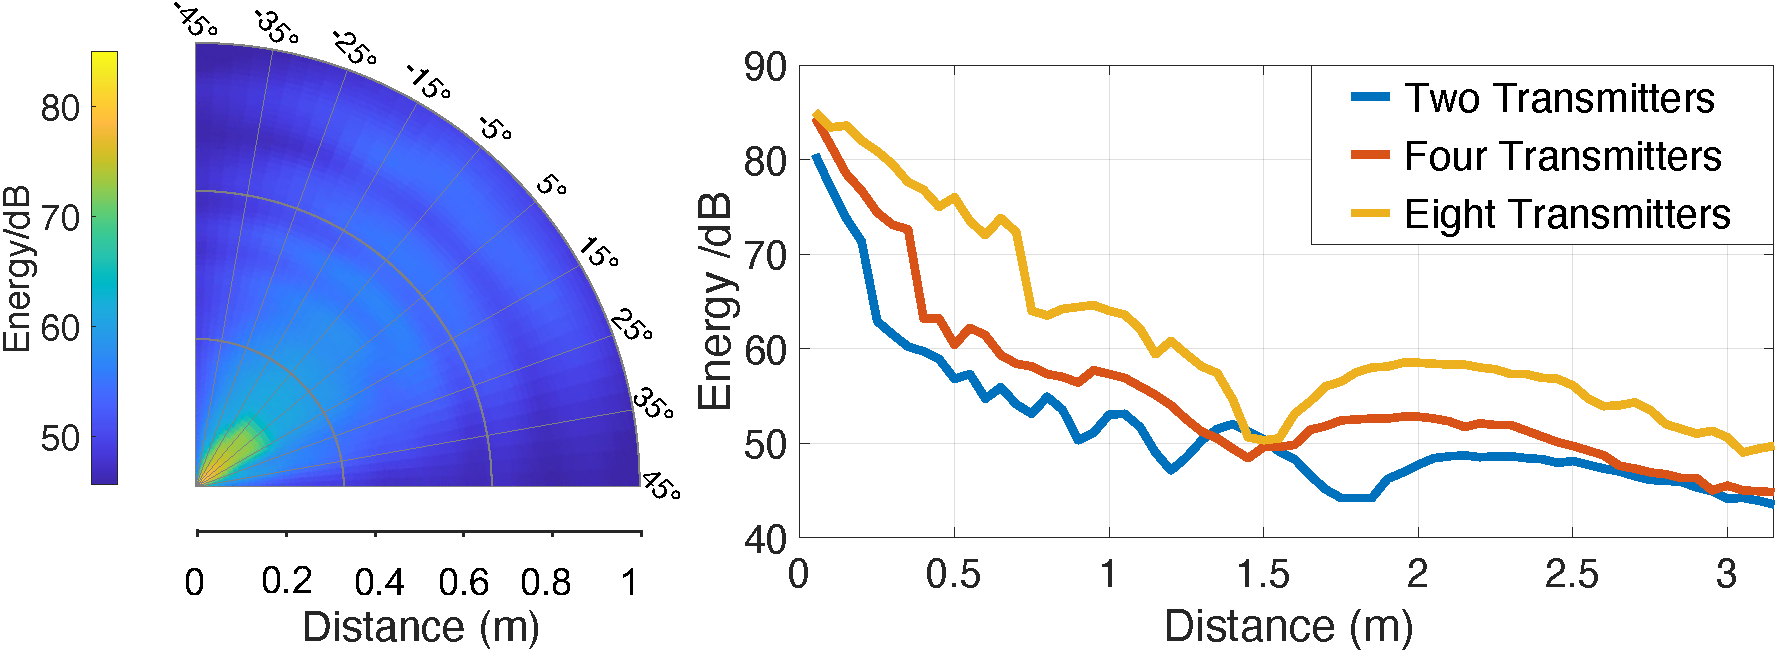
\includegraphics[width=\linewidth]{images/energy_distribution.pdf}
    \caption{Characteristics of the transmitter. Left: Energy distribution of two transmitters. Right: Energy attenuation with distance when the angle is $0^\circ$.}
    \label{fig:energy_distribution}
    \vspace{-5mm}
\end{figure}


\subsection{Transmitter Array Design}
 To extend the coverage of the transmitter, we design a transmitter array as shown in Figure~\ref{fig:transmitter_array}~(left). We install transmitters in a hexagonal shape on the spherical foam and separate them into two groups: one group sends the carrier signal and the other sends the modulated noise signal. The curvature of the spherical foam and the distribution of the transmitters enable the large coverage of the transmitter array. The energy distribution around the transmitter array is shown in Figure~\ref{fig:transmitter_array}~(right) and it is obvious that it can cover a large span of angle up to about $90^{\circ}$ and a much longer distance compared to using a single transmitter.

\begin{figure*}
    \centering
    \begin{minipage}[t]{0.75\textwidth}
        \begin{subfigure}[t]{0.51\linewidth}
            \begin{subfigure}[b]{0.3\linewidth}
                \centering
                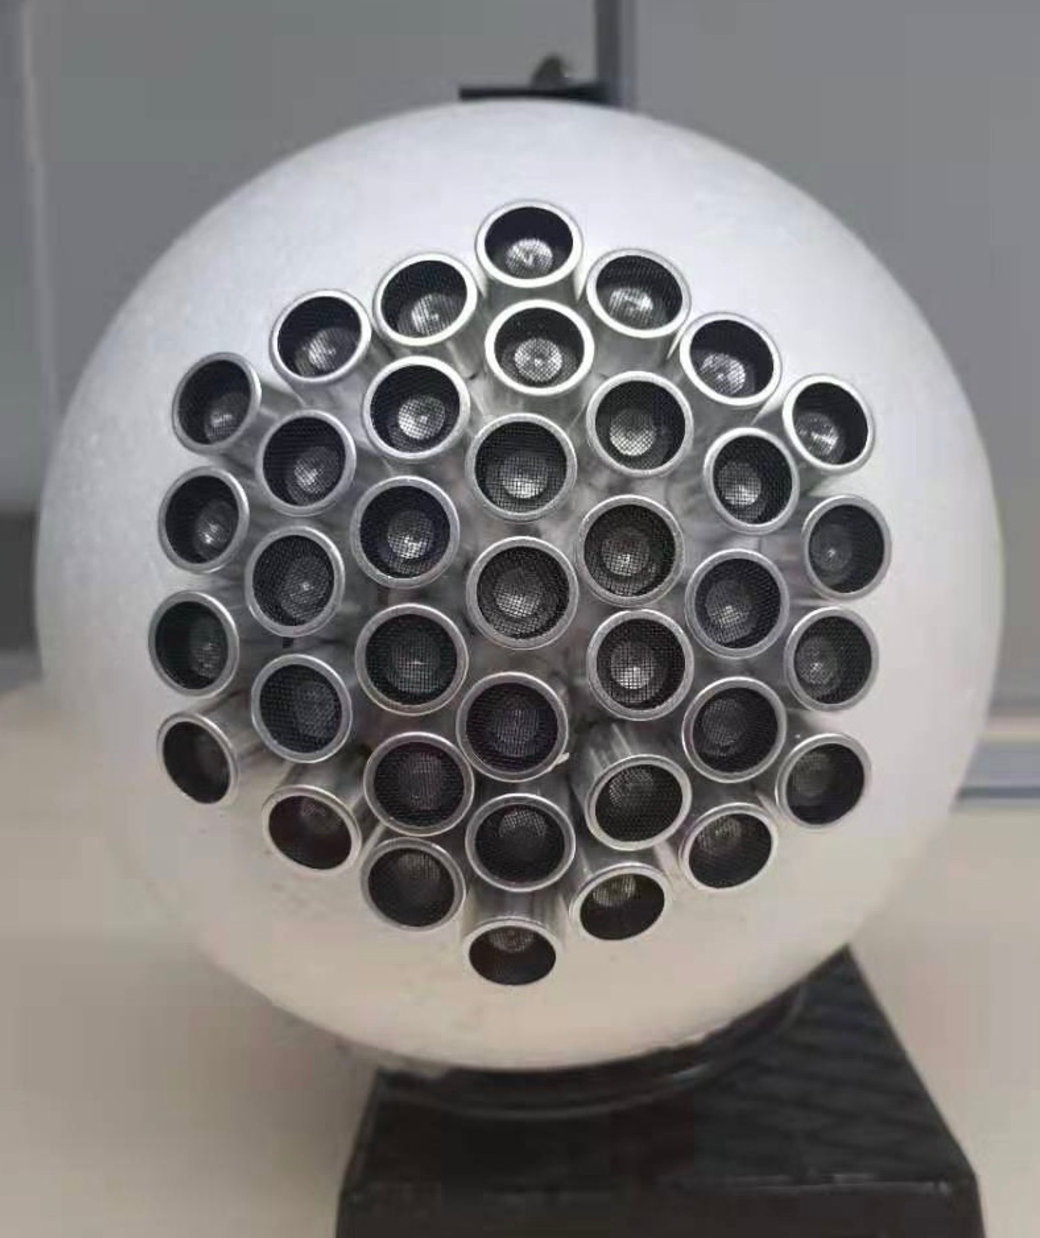
\includegraphics[width=\linewidth]{images/transmitter/transmitter.pdf}
            \end{subfigure}
            \begin{subfigure}[b]{0.3\linewidth}  
                \centering 
                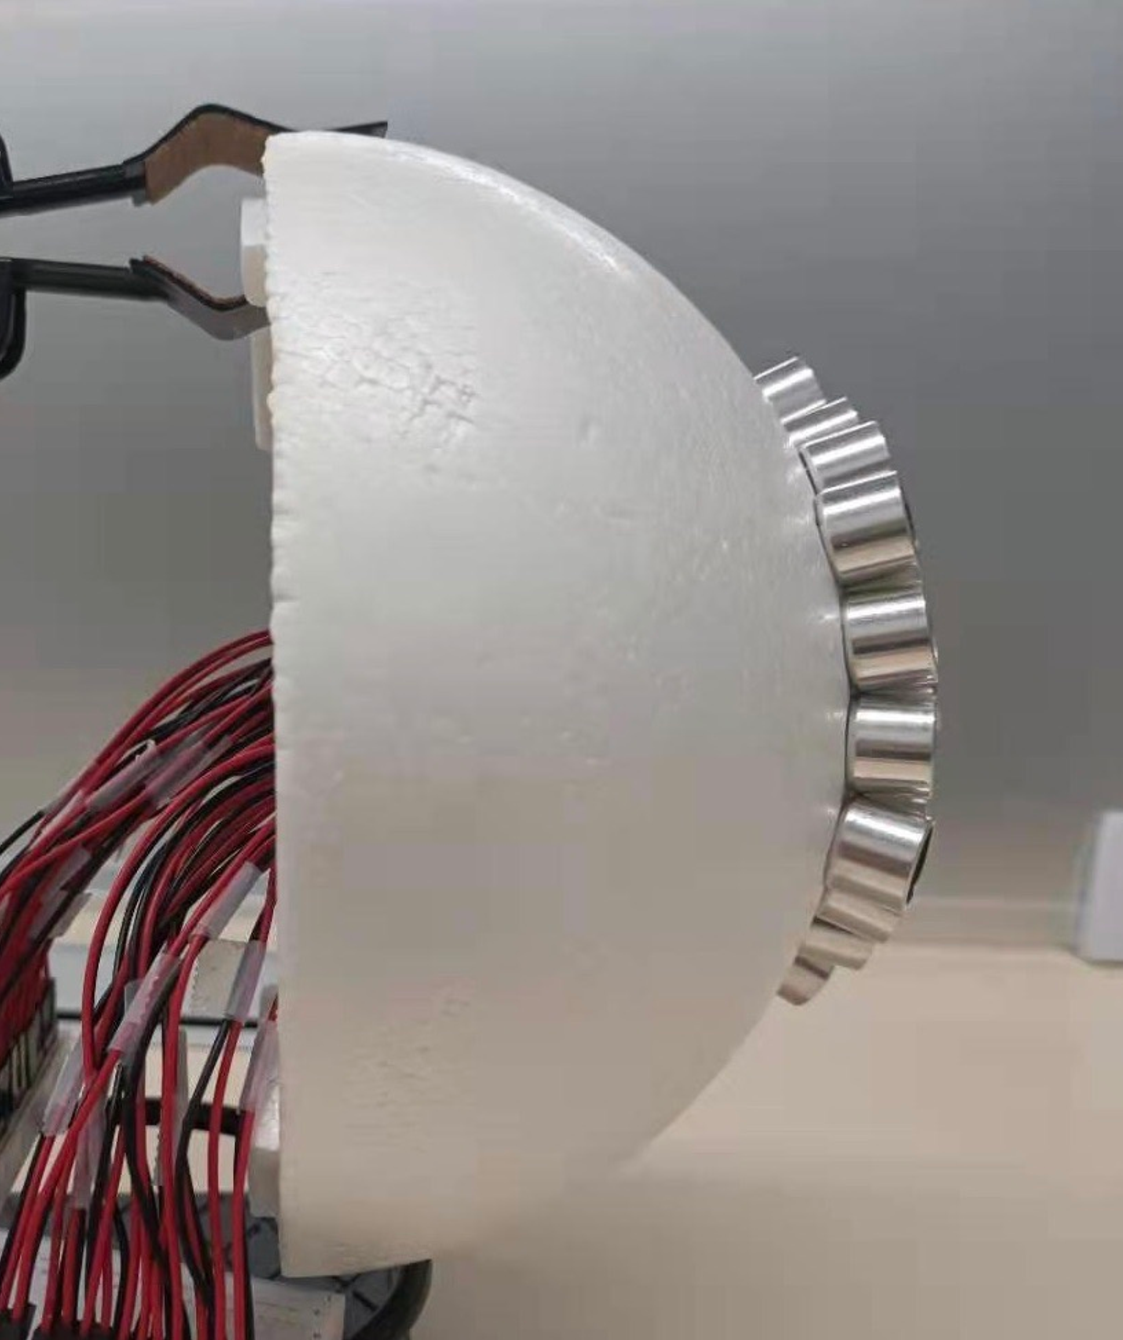
\includegraphics[width=\linewidth]{images/transmitter/transmitter_side.pdf}
            \end{subfigure}
            \begin{subfigure}[b]{0.3\linewidth}   
                \centering 
                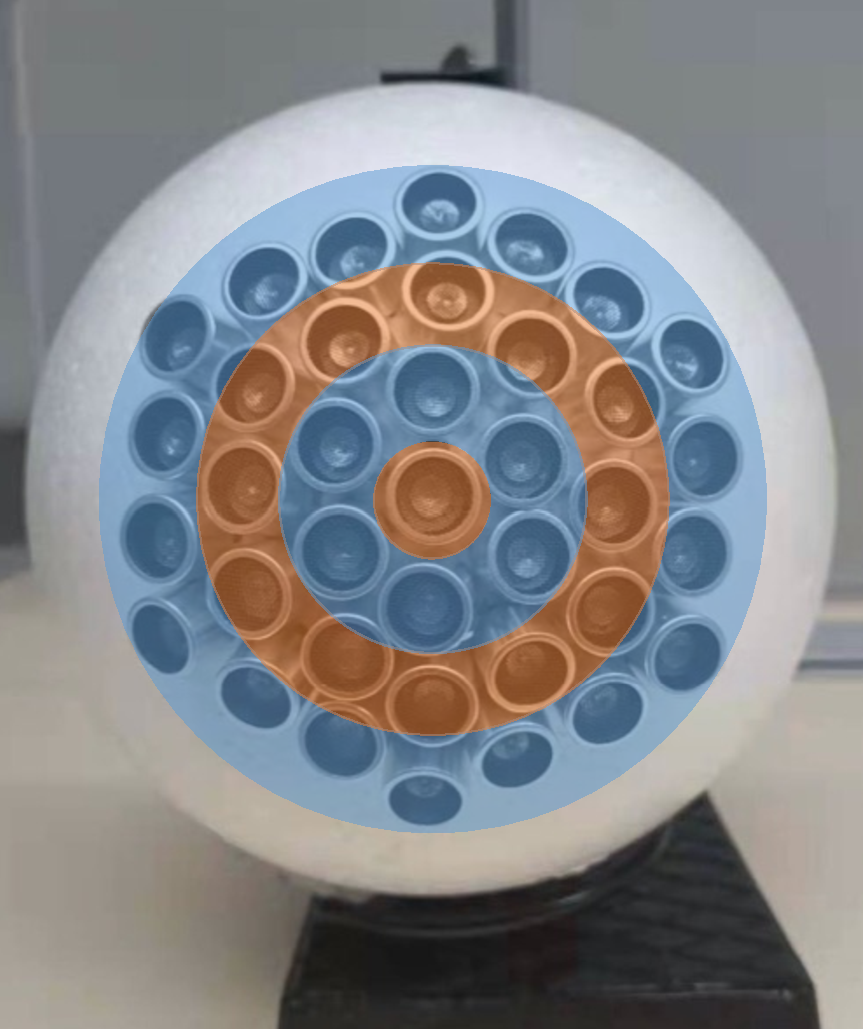
\includegraphics[width=\linewidth]{images/transmitter/separate.pdf}
            \end{subfigure}
            % \caption{}
            % \label{fig:transmitter_overview}
        \end{subfigure}
        \begin{subfigure}[t]{0.44\linewidth}
            \centering
            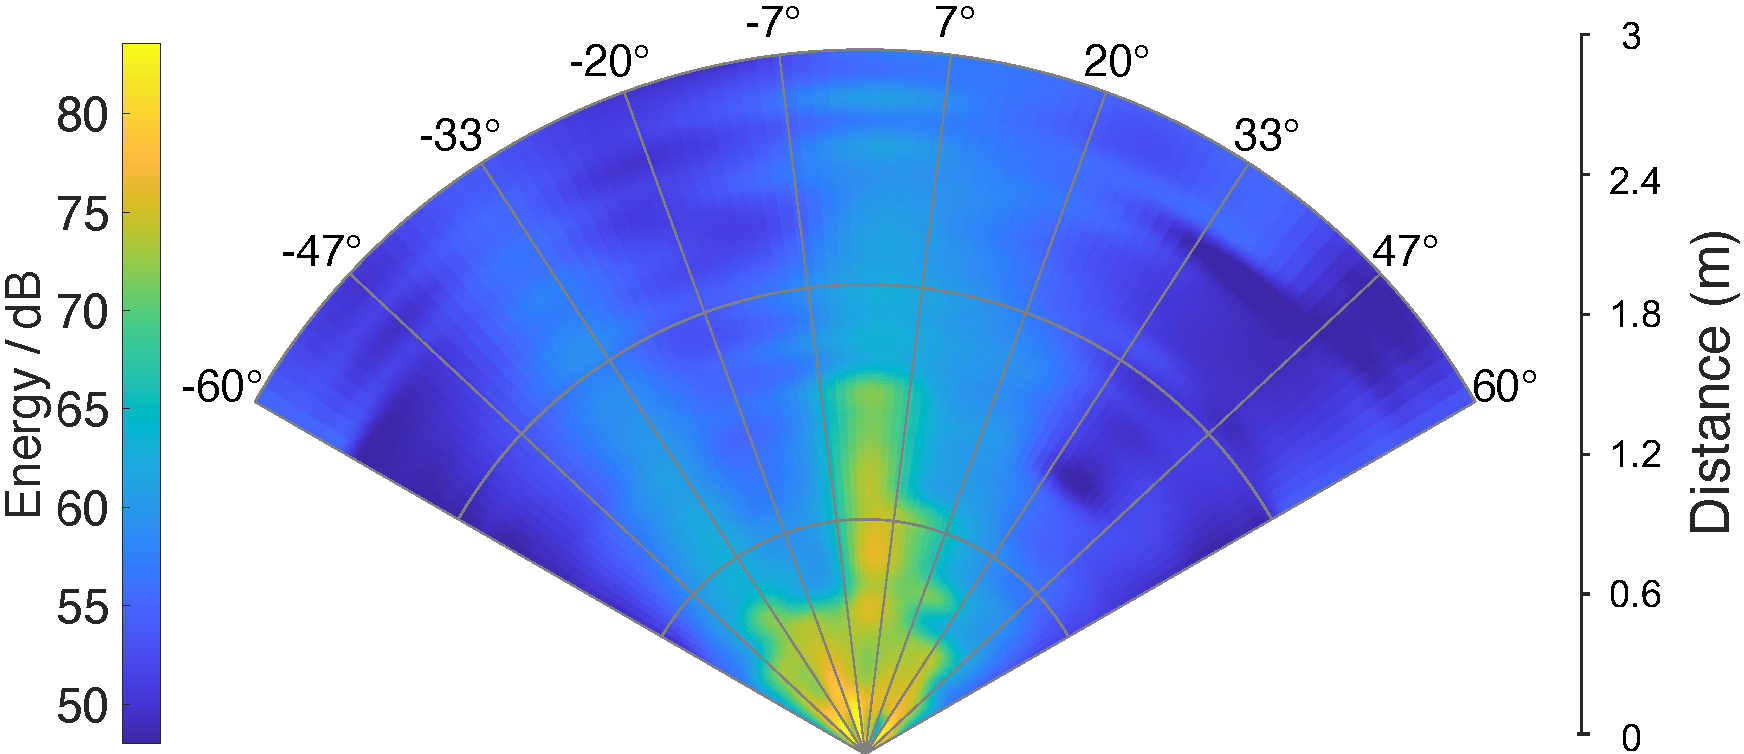
\includegraphics[width=\linewidth]{images/array_distribution.pdf}
            % \caption{}
            % \label{fig:array_distribution}
        \end{subfigure}
        \caption{The transmitter array. Left: The orange transmitters transmit the carrier signal while the blue ones transmit the modulated noise signal. Right: Energy distribution of the array}
        \label{fig:transmitter_array}
    \end{minipage}
    \begin{minipage}[t]{0.23\textwidth}
        \centering
        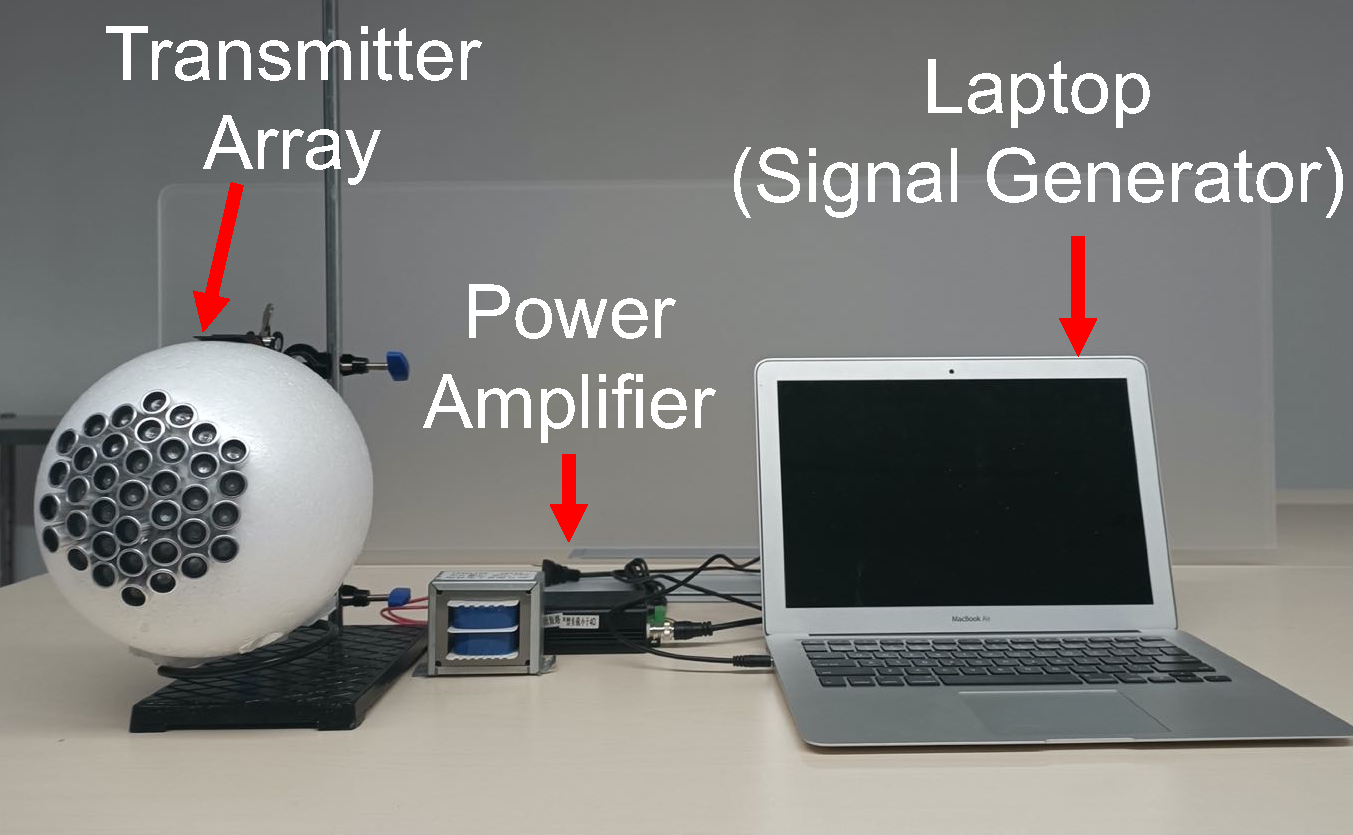
\includegraphics[width=\linewidth]{images/equipment.pdf}
        \caption{Hardware implementation.}
        \label{fig:hardware_implementation}
    \end{minipage}
    \vspace{-5mm}
\end{figure*}

\subsection{Hardware Implementation}
The implementation is shown in Figure~\ref{fig:hardware_implementation}, including a transmitter array, two power amplifiers (one for each transmitter group), a signal generator ( We use a laptop here but it could be replaced by other development boards with a sound card sampling rate $\geq$ 80kHz). The content recovery is realized on a backend server (Intel(R) Xeon(R) Gold 6226R CPU and a Nvidia RTX3090 GPU in this paper). Without considering the laptop and the backend server, the hardware implementation costs about 70 dollars. 